\chapter{CP, SAT and SMT}
\label{cha:CS}
\label{CS:Intro}
\label{CS:HolyGrail}
\section{Holy grail of programming}
\begin{quote}
	"Constraint programming represents one of the closest approaches computer science has yet made to the Holy Grail of programming: the user states the problem, the computer solves it." 
	\newline
	-Eugene C. Freuder in "In Pursuit of the Holy Grail" \cite{11freuder1997pursuitHolyGrail}.
\end{quote}
As the quote and the paper \cite{11freuder1997pursuitHolyGrail} from Eugene C. Freuder says, he and others believe that in the ideal world the user conveys any problem to a computer or a program and that the program will solve it. Which matches a coarse summary of what a constraint programming language (CP) can do in an ideal world. But we do not live in that type of world and problems need to be converted or split up into a representation that the solver can understand. 
This is where constraints come into the picture, constraints are mathematical, logical or relational connections put on or between variables to form a model that hopefully satisfy all constraints after solving. This is sometimes combined with a final objective function to be minimized or maximized, for example finding a model where a postman visits all cities on a route but with a minimal distance traveled. 
With CP the focus lays more on the solving high level problems with specialties around scheduling and planning \cite{52bartak1999constraint}. CP's key feature being the global constraints, a set of "functions" that are aimed at a high level of solving. For example, the "alldifferent()" which makes sure that all variables within an array will be assigned a different value or "circuit()" that holds if the input forms a Hamiltonian circuit.

A second field of research that we will discuss is the boolean satisfiability problem better known as SAT, where the focus lays on the boolean variant of constraints within the family of constraint solvers. This field of research has produced quite a lot of progress due to its age, resulting in efficient solving \cite{56bardin2019bringing}.

Our last field, is the satisfiability modulo theory (SMT) which builds further on SAT. This by including lists, arrays, strings, real numbers, integers and other more complex data structures and types. With SMT the focus lays more on static checking and program verification \cite{56bardin2019bringing, 54moura2008z3}.


\section{Constraint programming}
\label{CS:CP}
As mentioned before CP's are well versatile in the solving of constraints and especially when it comes to planning and scheduling. This by their efficient constraint propagation, backtracking and the linking of related constraints \cite{66WikiCP}. Originally CP's can be linked back to constraint logic programming (CLP) where programming languages (mostly logic programming languages) where combined with constraints and ways to solve them. A notable version is that of Joxan Jaffart and Jean-Louis Lassez \cite{65jaffar1987constraint, 66WikiCP} with their extension in Prolog and thereby the creation the category.

To further introduces you to constraint programming we will show a popular puzzle in the CP field "send more money". which is a logic puzzle made by Henry Dudeney and published in Strand Magazine's July 1924 edition \cite{sendMoreMoney}.
In this puzzle each character represents a single digit between zero and nine (both included), meaning that the 'e' from "send" should be the same digit as the 'e' from "more" and the 'e' from "money". The other rules go as follows: all different characters should have a different digit, any of the starting letter of each word cannot be zero and after replacing all characters with their corresponding digits the sum should be correct. 
\begin{center}
	\[$$
	\; \; S E N D\\
	+ M O R E\\
	-----------------\\
	M O N E Y
	$$\] The "send more money" puzzle.
\end{center}
On top of showing the problem we will also use MiniZinc\footnote{\url{https://www.minizinc.org/}} as our constraint programming language to find the solution for this puzzle. By doing this we will show a possible representation of this problems using constraints so that a solver can find a solution.

\label{lst:SendMoreMoney}
\begin{lstlisting}[float=t,language=minizinc, caption={Solution to the puzzle "send more money" slightly modified from \url{https://www.minizinc.org/doc-2.5.5/en/downloads/send-more-money.mzn}}]
	include "globals.mzn";
	var 1..9: S; % Since 'S' is a starting character it is limited from 1 to 9.
	var 0..9: E; % Other characters are limited from 0 to 9.
	var 0..9: N;
	var 0..9: D;
	var 1..9: M;
	var 0..9: O;
	var 0..9: R;
	var 0..9: Y;
	
	constraint % The sum must hold.
	              1000 * S + 100 * E + 10 * N + D
	            + 1000 * M + 100 * O + 10 * R + E
	= 10000 * M + 1000 * O + 100 * N + 10 * E + Y;
	
	constraint alldifferent([S,E,N,D,M,O,R,Y]);
	
	solve satisfy;
	output % Pretty-printing the solution.
	[" \(S)\(E)\(N)\(D)\n",
	"+ \(M)\(O)\(R)\(E)\n",
	"= \(M)\(O)\(N)\(E)\(Y)\n"];
\end{lstlisting}
\label{sendMoreMoneyExplanation}
On line 1 you can see the importing of the global constraints, which CPs are known for. Line 2 until 9 we can see the declarations of all possible characters to the possible digits, starting letters such as 'S' and 'M' are limited by their representation from 1 to 9 instead of using a constraint. The constraint on line 11 runs through until line 14, where it is closed by the semicolon. This constraint specifies the matching of the sum. At line 16 we use one of the imported functions namely "alldifferent()" which will satisfy if no duplicate values occur in the array. To then start solving for satisfiability at line 18, this in comparison of solving for minimization or maximization an objectify function, which does not apply here. Finally, after a solver has found a solution we print the result using a pretty-print from line 19 to 22.
We will not be spoiling the solution and will leave it up to you to find the solution but remember that you can check your answer with the program above.

The "alldifferent()" and the sum constraint also show us the power of CPs, with a single statement multiple relations are expressed \cite{53marriott1998programming}. Instead of needing to specify all possible relations of the last three characters of each word (\mbox{D + E = Y}, \mbox{Y - D = E} and \mbox{Y - E = D}) a single expression suffices. When knowing two values we can infer the third, imagine the work needed for the "alldifferent()" constraint. The developer would have to go over all possible combinations, this in combination of specific smart back-end solvers for this constraint makes MiniZinc and other CP-solvers so powerful. 

\subsection{origin}
Within constraint programming we can distinguish two branches \cite{52bartak1999constraint}: one being constraint satisfaction. Which puts the focus on finding a model which satisfies all constraints. which can be done with generating values within the domain of the variables and testing them, also called generate and test but obviously this is not the fastest way. 

On the other hand, we have constraint optimization, which covers an even harder problem. Instead of having to check if all constraints satisfy, here we want to know what model will give us the highest or lowest value. The function to optimize is often called the objective function and occurs more often than not in real life problems \cite{52bartak1999constraint}. 
Unfortunately depending on the problem, we regularly hit limitations due to NP-hardness. This has challenged the field and multiple different search strategies to gain a higher efficiency have been thought off. Popular approaches to finding solutions in both branches are the use of constraint propagation, backtracking, symmetry breaking, dynamic programming, techniques from the CP solvers like lazy clause generation and even heuristics as: local search, Tabu search, simulated annealing and more. 

\subsection{MiniZinc}
A keen observer has will have noticed that we used "after \underline{a} solver has found satisfiability" in the explanation of "send more money" in section \ref{sendMoreMoneyExplanation}. 
This is because MiniZinc is not a solver, it came to be from the lack of standard modeling language surrounding CP's. Before MiniZinc, when you wanted to use another solver, you had to rewrite your problem again in that solver's specific language. This is what Nicholas Nethercote et al. wanted to solve, they came up with MiniZinc, which is a modeling language for CPs that is not connected to a single specific solver \cite{57nethercote2007minizinc}. It originated from a modeling language focused on constraints, called Zinc \cite{68incbanda2006modelling} and as you can tell by its name MiniZinc, it is a subset of Zinc \cite{57nethercote2007minizinc}.
In the words of Peter J. Stucke, a member of the MiniZinc team: 

\begin{quote}
	"MiniZinc is high level enough to express most combinatorial optimization problems easily and in a largely solver-
	independent way; (...) However, MiniZinc is low level enough that it can be mapped easily onto many solvers." 
	\newline
	-Peter J. Stuckey et al. in "The MiniZinc Challenge 2008-2013" \cite{58stuckey2014minizinc}.
\end{quote} which shows the team's vision of MiniZinc.

MiniZinc transforms its inputs to FlatZinc by combining the model, data and solver specific features. Which then can be solved by a specific solver. The list of CP solvers that support MiniZinc, at the time of writing 17 solvers have FlatZinc interfaces.

\subsubsection{MiniZinc Challenge}
On top of maintaining and improving MiniZinc the MiniZinc team also organizes a yearly challenge to compare and test what improvements have been made in the constraint solving world. Which they are able to do by having the benefit of a standardized constraint programming language to benchmark with. 
In this yearly challenge each solver gets fifteen minutes to solve a hundred selected problem instances. But due the difficulty of having to find quite a number of good representative problem instances each year, the organizers of the challenge ask the participants to submit preferably two problem models and multiple related instances. From the received list the jury then tries to make a fair selection to cover the use of global constraints, real-world representative problems, to find a good balance between satisfying versus optimization problems and the different types of technologies (SAT and MIP) instead of only selecting CP focused problems \cite{58stuckey2014minizinc}.

It is due to this MiniZinc challenge that a better connection has formed between CP solvers and SAT solvers. By attracting SAT solvers to the challenge, tools such as fzn2smt \cite{72bofill2010system} and BEE \cite{69BEEmetodi2012compiling} arose. These tools are able to translate FlatZinc to SAT-LIB and conjunctive normal form (CNF) respectively. 
With BEE producing CNF, Amit Metodi and Michael Codish where then able to let a SAT solver solve the problem. Although the latter is limited to finite domain constraint problems, it allows utilization of large and swift SAT-solvers on top of bringing the field of research closer to each other.

On top of being a great way to benchmark comparative solvers the MiniZinc challenge, it also results in more solver implementing the FlatZinc as an input and due to the competitive nature of academics brings the motivation to stride forwards according to the author of "Philosophy of the MiniZinc challenge", Julien Fischer \cite{59stuckey2010philosophy}.

\subsection{CPMpy}
\label{CP:CPMpy}
MiniZinc is not de only one with the idea to create a modeling language for CPs, other examples are Essence with the focus on combinatorial problems for people with a background in discrete mathematics \cite{70frisch2008essence}.
And the one with our most interest is the constraint programming and modeling language for Python (CPMpy). Based around the popular packet NumPy, CPMpy allows for a lower learning curve of constraint programming languages by creating a constraint programming and modeling language in a familiar language \cite{17guns2019increasing}. 
With NumPy comes with a lot of advantages: it is popular in data processing and the general array-based operations among machine learning and more. 
Being able to use these in combination of CPs would allow for both fields to grow closer to each other. 


At the time of writing the CPMpy has support for multiple solvers like OR-tools, CP-SAT, Gurobi (for MIP problems), PySAT (which is a library that contains 13 different SAT solvers), PySSD which is a knowledge compiler and CPMpy has support for any CP-solver that support for the text-based MiniZinc language \cite{CPMpyDoc, CPMpyGithub} (resulting in at least 33 extra solvers). With potential future extensions to Microsoft's Z3 theorem prover and others as new solvers.
We would have written an in-depth explanation on how CPMpy does its conversions from constraints to what is given to the solvers, but CPMpy being in development and with more changes potential coming this could become outdated quickly. We look forward to see CPMpy progress and the future paper(s) discussing it. What we can do is discuss it on a global level, where we see CPMpy existing out of four components. This being a model part (everything to do with creating a model of a problem), a transformation part (everything to do with changing constraints), solver specific part transformations (everything to do with restrictions the solver puts on CPMpy) and then the solver themselves (which solve the final model). With CPMpy having little to no control over the last one as can be seen in figure \ref{fig:4ComponentsOfCPMpy}.


Finally, to illustrate that both MiniZinc and CPMpy are not that far apart we included a CPMpy listing (listing \ref{lst:SendMoreMoneyCPMpy}) for the same problem as we have seen for MiniZinc.

\begin{figure}
	\centering
	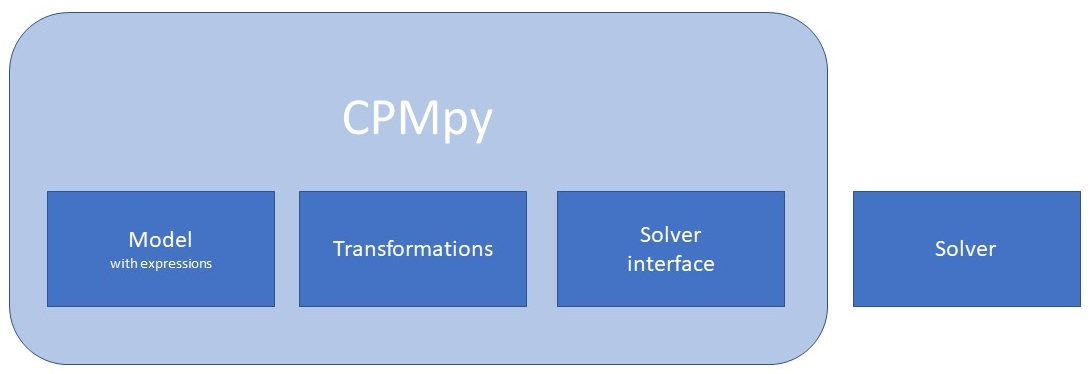
\includegraphics[width=1.0\textwidth]{images/4componentsOfCPMpy}
	\caption{The four main components of CPMpy}
	\label{fig:4ComponentsOfCPMpy}
\end{figure}


\label{lst:SendMoreMoneyCPMpy}
\begin{lstlisting}[float=, language=python, caption={Solution to the puzzle "send more money". Modified from the example in the CPMpy repository \url{https://github.com/CPMpy/cpmpy/blob/master/examples/send_more_money.py}}]
	#!/usr/bin/python3
	"""
	Send more money in CPMpy
	  SEND
	+ MORE
	------
	 MONEY
	"""
	from cpmpy import *
	import numpy as np
	
	s,e,n,d,m,o,r,y = intvar(0,9, shape=8) # creating variables
	
	model = Model() # with "+=" we can add a constraint to the model
	model += sum([s,e,n,d] * np.array([1000, 100, 10, 1])) \
	       + sum([m,o,r,e] * np.array([1000, 100, 10, 1])) \
	      == sum([m,o,n,e,y] * np.array([10000, 1000, 100, 10, 1]))
	model += AllDifferent([s,e,n,d,m,o,r,y])
	model += s > 0 # in MiniZinc each variable was declared seperatly in CPMpy 
	model += m > 0 # we can do it in batch, resulting in these extra constraints 
	
	print(model)
	
	# Solve and pretty-print
	if model.solve():
	   print("  S,E,N,D =   ", [x.value() for x in [s,e,n,d]])
	   print("  M,O,R,E =   ", [x.value() for x in [m,o,r,e]])
	   print("M,O,N,E,Y =",    [x.value() for x in [m,o,n,e,y]])
	else:
	   print("No solution found")
\end{lstlisting}
%We have shortly seen how a CPMpy looks like in listing \ref{lst:SendMoreMoneyCPMpy}, 
%where we create a model, add constraints to it and then to solve the model. Everything up to the solving part is controlled by CPMpy, once the "solve()" is called 


% where errors could occure, whitch ones are in/out of scope

\section{SAT}
\label{CS:SAT}
Now that we discussed CPs, let's step back to boolean satisfiability problems (SAT) and as the name already spoiled it, here we are focused on checking the satisfiability of boolean formulas. SAT has been successful in the hardware design and verification. With al lot of research in improving SAT-solvers, they have become significant efficient on large problems \cite{56bardin2019bringing}.
With the efficiency improvements coming from the DPLL algorithm to conflict-driven clause learning (CDCL) move combined with the addition of non-chronological back jumps. But better propagation, lazy clause generation (LCG), data structures and the introduction of heuristics assisted significantly to the process. Heuristics often include clause deletion to decrease the number of unused clauses, variable state independent decaying sum (VSIDS) where we add a decaying weight (the sum) to select which literal we prioritize, random restarts where we try to avoid large search trees by restarting with the learned clauses, among other heuristics \cite{61MCSMarcDenecker, 60katebi2011empirical, 67stuckey2010lazyClauseGeneration}.
%more techniques: branching, unit propagation, backtracking, 2 watched literals, heuristics: detpth, breadth first, Variable state independent decaying sum/VSIDS, dynamic largest individual sum (DLIS), clause deletion, random restarts

%\todo{example?}


\section{SMT}
\label{CS:SMT}
An extension of SAT is satisfiability modulo theories (SMT), which extends the only boolean focus of SAT with quantifiers, integers, lists, arrays and much more. With the advantage that most efficient algorithms from SAT transfers over. The focus with this technology lays in multiple fields but it is quite popular in program verification and testing. As can be seen with Microsoft's Z3\footnote{\url{https://github.com/Z3Prover/z3}}, which is focused on static software checking \cite{54moura2008z3}. Z3 is one of the most popular SMT theorem provers at the moment, with a considerable number of varying supported theories. It has support for the standard SMT-LIB input, the simplify input (from an older theorem prover) \cite{73detlefs2005simplify}, and a low-level native input for textual input-based directly. Z3 also has APIs for the following programming languages: C/C++, .NET, OCaml, Python, Java, Haskell and more \cite{64WikiSMT}.

The second most popular SMT-theorem prover is from the cooperating validity checkers (CVC) line-up. The latest in the CVC-lineup is CVC5\footnote{\url{https://github.com/cvc5/cvc5}}, which is the fifth in line of the CVC-family, the previous being: SVC (not always counted), CVC, 
CVC Lite\footnote{\url{https://cs.nyu.edu/acsys/cvcl/}}, 
CVC3\footnote{\url{https://cs.nyu.edu/acsys/cvc3/}}\cite{71barrett2007cvc3} and 
CVC4\footnote{\url{https://cvc4.github.io/}}.
As like CVC4, CVC5 supports the standard SMT-LIB input format among other formats directly and has APIs for C++, Python, Java and probably more by the time you read this \cite{62barrettcvc5, 63barbosa2022cvc5}.

\section{Conclusion}
\label{CS:conclusion}
In this chapter we discussed some of the most popular parts of constraint solving. We explain the boolean constraints within SAT to be able to better explain the broader non-boolean constraints within SMT and constraint programming. On top of that have also seen multiple tools used in the industry and academia to prove and/or solve constraint problems.

%%% Local Variables: 
%%% mode: latex
%%% TeX-master: "thesis"
%%% End: 
